\documentclass[12pt]{article}

% ---------- Packages ----------
\usepackage[margin=1in]{geometry}   
\usepackage{graphicx}               
\usepackage{amsmath, amssymb}      
\usepackage{booktabs}               
\usepackage{hyperref}             
\usepackage{float}                  
\usepackage{caption}               
\usepackage{xcolor}                 
\usepackage{tikz}
\usetikzlibrary{positioning, arrows.meta, fit}

\usepackage[
    backend=biber,
    style=apa,
    citestyle=authoryear,
]{biblatex}
\addbibresource{refs.bib}



\hypersetup{
  colorlinks=true,
  linkcolor=blue,
  citecolor=blue,
  urlcolor=blue
}

\title{\textbf{Inferring Cuba's Hidden Economy: A Bayesian Latent Variable Model}}
\author{Christopher M. Perez}
\date{May 13, 2025}

\begin{document}
\maketitle
\tableofcontents
\newpage

\section{Introduction}
\label{sec:intro}

Measuring economic well-being in Cuba is notoriously difficult due to scarce and unreliable official statistics. The World Bank's open data portal lacks many poverty and inequality metrics for Cuba, and even basic metrics like GDP growth are contested---recent figures suggest an annual growth rate of just 1.4\% \parencite{worldbankcuba}. In the absence of trustworthy ground data, researchers increasingly turn to satellite-based proxies. Nighttime lights, for example, strongly correlate with economic output in data-sparse regions, and Cuba's contrast to  Florida in nighttime imagery highlights its economic constraints \parencite{steele2017poverty}.

In light of these data limitations, I adopt a Bayesian latent variable model to estimate a subnational index of economic activity in Cuba using three high-resolution proxies: nightime lights (VIIRS), normalized difference vegetation index (NDVI), and road density. This latent factor framework allows us to infer relative economic activity even without traditional survey data. Results are then cross-validated in the Dominican Republic (DR), where data is easily accessible, thereby providing a systematic method for mapping economic activity in data-poor settings.


\section{Data and Preprocessing}

I utilize three geospatial proxies for economic activity in Cuba, all aligned on a 500 m grid, that capture different aspects of development. All data correspond to the 2024 year.

\label{sec:data}
\begin{itemize}
  \item \textbf{Nighttime Lights (VIIRS):} Satellite-measured night light intensity, a well-known proxy for economic output. Brighter areas tend to indicate higher population density, infrastructure, and GDP.
  \item \textbf{NDVI (Vegetation):} The Normalized Difference Vegetation Index captures “greeness.” While high NDVI often signifies productive agriculture or healthy ecosystems, it can also be inversely correlated with poverty in some contexts.
  \item \textbf{Road Density (OpenStreetMap):} Measures the density of roads, reflecting infrastructure. Well-connected regions tend to be more economically active.
\end{itemize}

All layers are reprojected and aligned to the same grid, and masked to exclude water or uninhabited zones. Each proxy is then standardized to account for different scales.

\section{Bayesian Hierarchical Model}
\label{sec:model}

We define a latent variable $z_i$ for each grid cell $i$, representing the underlying economic activity (on an arbitrary scale). The observed proxies are linked to $z_i$ via a linear model described below.

\subsection{Observation Model}
For grid cell~$i$ and proxy~$k$, let 
\[
x_{i,k} \;\sim\; \mathcal{N}\!\bigl(\beta_k\,z_i,\;\sigma_k^2\bigr),
\qquad
k \in \{\text{lights},\;\text{NDVI},\;\text{roads}\},
\]

where $\beta_k$ is a weight and $\sigma_k$ is the standard deviation for proxy $k$. This implies that each proxy is a noisy linear indicator of the same latent $z_i$. For example, nighttime light intensity $x_{i,\text{lights}}$ is modeled as: $z_i \cdot \beta_{\text{lights}} + \text{noise}$.

\subsection{Identifiability Constraint}
To address the identifiability issue, I fix $\beta_{\text{lights}}=1$, a unit coefficient on lights. This anchors the latent scale such that an increase of 1 in $z$ corresponds to one standard deviation increase in night lights. 

The other coefficients have weakly informative priors: $\beta_{\text{NDVI}},\,\beta_{\text{roads}} \sim \mathcal N(0,1)$. This allows NDVI and road density to be learned as either positive or negative indicators of $z$. 


\subsection{Spatial ICAR Prior and Neighborhood Smoothing}

In our model, we include a spatial random effect modeled with an Intrinsic Conditional Auto-Regressive (ICAR) prior. This prior introduces spatial smoothing by enforcing that neighboring areas have similar random-effect values. This is achieved using the adjacency matrix of the grid cells, which is a square matrix where each element $A_{ij}$ is 1 if cell $i$ and cell $j$ are neighbors and 0 otherwise. Under this prior, each area's effect is conditioned on the average of its neighbors' effects. In practice, we add a prior potential
\[
\;\propto\;
\exp\!\left\{-\frac{\tau}{2}\sum_{(i,j)\in\mathcal N}(z_i-z_j)^2\right\},
\]
where $\mathcal N$ is the set of neighbor pairs, and where $\tau$ is the spatial precision parameter \parencite{duncan2017spatial}. 

The advatange of using an ICAR prior is the localized smoothing it provides. The model will produce more reliable estimates for each area by pooling information with its neighbors. This is especially helpful for areas with sparse data. Additionally, it also maintains local distinctness in that each area is mainly informed by its immediate neighbors, rather than enforcing a single global effect.

A concern with ICAR is the issue of spatial confounding, which occurs when a spatially-structured random effect competes with or masks the effects of spatially correlated covariates. In our analysis, we remain mindful of this issue so that it does not inadvertently obscure the estimated effects of our proxies.


\subsection{Weakly Informative Priors}

The spatial precision $\tau$ and the standard deviations $\sigma_k$ parameters are modeled using weakly informative priors. Specifically $\tau, \sigma_k \sim \text{HalfNormal}(1)$. This choice allows us to have some regularization: it provides some information to prevent extreme or implausible values of the variance parameters without being too strongly constraining. This also helps improve convergence and guard against overly diffuse posteriors without contributing too much bias \parencite{gelman2006prior}.


Moreover, we use a non‑centered parameterization $z_i = \dfrac{z_i^{\mathrm{raw}}}{\sqrt{\tau}}$, where $\; z_i^{\mathrm{raw}}\sim\mathcal N(0,1)$, to decouple the highly correlated magnitude of $z$ and $\tau$.


\begin{figure}[H]
  \centering
  \resizebox{0.85\textwidth}{!}{ % Adjust width scale here
  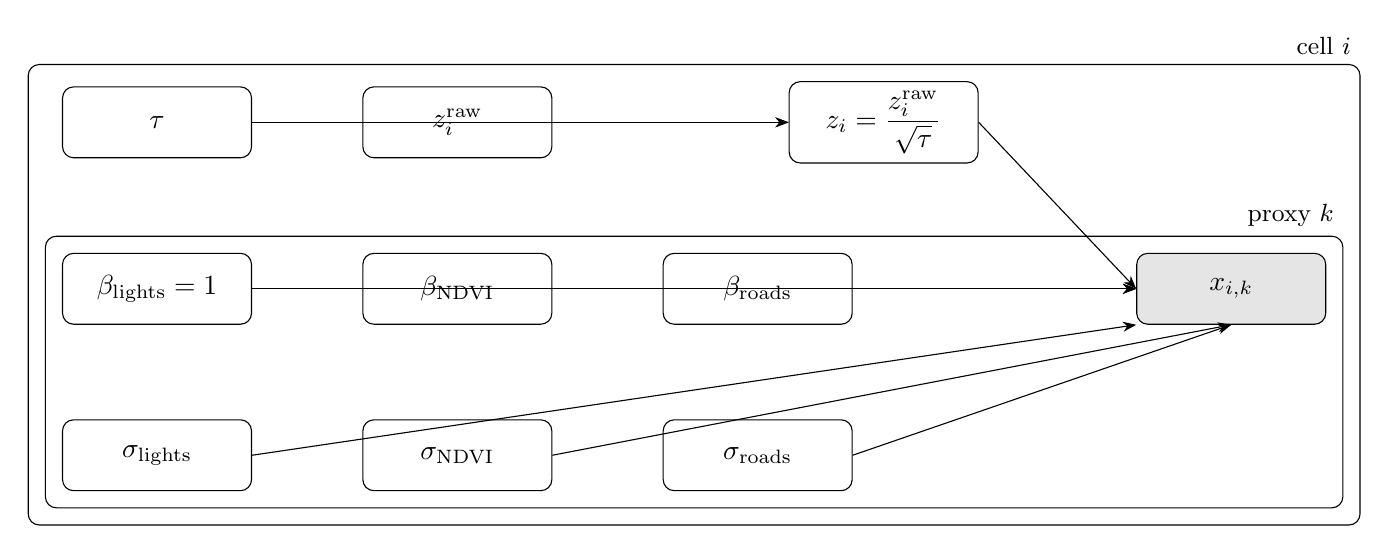
\begin{tikzpicture}[
      node distance = 12mm and 14mm,
      latent/.style  = {draw, rounded corners, minimum width=24mm, minimum height=9mm},
      param/.style   = {draw, rounded corners, minimum width=24mm, minimum height=9mm},
      obs/.style     = {draw, rounded corners, fill=gray!20, minimum width=24mm, minimum height=9mm},
      plate/.style   = {draw, rounded corners, inner sep=6pt},
      >={Stealth[]}
  ]

  % --- Latent precision and raw field ---
  \node[param]  (tau)   {$\tau$};
  \node[latent, right=of tau] (zraw) {$z^{\mathrm{raw}}_i$};
  \node[latent, right=30mm of zraw] (z)
        {$\displaystyle z_i = \frac{z^{\mathrm{raw}}_i}{\sqrt{\tau}}$};

  \draw[->] (tau) -- (z);     
  \draw[->] (zraw) -- (z);    

  % --- Loadings (betas) ---
  \node[param, below left=of zraw] (betaL) {$\beta_{\mathrm{lights}} = 1$};
  \node[param, right=of betaL]     (betaN) {$\beta_{\mathrm{NDVI}}$};
  \node[param, right=of betaN]     (betaR) {$\beta_{\mathrm{roads}}$};

  % --- Noise scales (sigmas) ---
  \node[param, below=of betaL] (sigL) {$\sigma_{\mathrm{lights}}$};
  \node[param, right=of sigL]  (sigN) {$\sigma_{\mathrm{NDVI}}$};
  \node[param, right=of sigN]  (sigR) {$\sigma_{\mathrm{roads}}$};

  % --- Observed variable ---
  \node[obs, right=36mm of betaR] (xik) {$x_{i,k}$};

  % --- Arrows into x_{i,k} ---
  \draw[->] (z.east)  -- (xik.west);       
  \draw[->] (betaL.east) -- (xik.west);
  \draw[->] (betaN.east) -- (xik.west);
  \draw[->] (betaR.east) -- (xik.west);
  \draw[->] (sigL.east) -- (xik.south west);
  \draw[->] (sigN.east) -- (xik.south);
  \draw[->] (sigR.east) -- (xik.south);

  % --- Plates --------------------------------------------------
  \node[plate, fit=(betaL) (betaN) (betaR) (sigL) (sigN) (sigR) (xik)] (plateK) {};
  \node at (plateK.north east) [anchor=south east, font=\small] {proxy $k$};

  \node[plate, fit=(tau) (zraw) (z) (plateK)] (plateI) {};
  \node at (plateI.north east) [anchor=south east, font=\small] {cell $i$};

  \end{tikzpicture}
  } % end resizebox
  \caption{Graphical model of the Bayesian latent‐variable hierarchy.}
  \label{fig:gm_cuba}
\end{figure}


\section{Posterior Results for Cuba (15 km Grid)}

After fitting the model, we obtain the latent economic activity index $z_i$ across Cuba at a 15 km cell resolution. Figure \ref{fig:posterior_map_round1} shows the posterior mean of $z_i$ for each cell across Cuba. Higher $z$ values (yellow) correspond to greater inferred activity. As expected, the model highlights major urban centers like Havana and Santiago de Cuba, while rural interior regions show lower $z$, reconstructing a plausible economic landscape.

\begin{figure}[H]
  \centering
  \includegraphics[width=0.6\textwidth]{/Users/chrisperez/Desktop/stat288-finalproject/images/fig1.png}
  \caption{Estimated latent economic activity index $z_i$ across Cuba.}
  \label{fig:posterior_map_round1} 
\end{figure}


Figure \ref{fig:posterior_map_round1_uncertainty} presents the posterior standard deviation of the $z_i$, which is relatively low overall (0.04-0.06), indicating high confidence in estimates. Slightly higher uncertainty appears near Havana particularly, while remote areas exhibit uniformly low uncertainty.

\begin{figure}[H]
  \centering
  \includegraphics[width=0.6\textwidth]{/Users/chrisperez/Desktop/stat288-finalproject/images/fig2.png}
  \caption{Estimated latent economic activity index $z_i$ across Cuba.}
  \label{fig:posterior_map_round1_uncertainty} 
\end{figure}


The learned coefficients reveal how each proxy contributes to $z$ (Figure \ref{fig:marginal_posterior_plot}). The NDVI coefficeint is modest, with $\beta_{\text{NDVI}} \approx 0.143$, while roads have the strongest influence, with $\beta_{\text{roads}} \approx 2.289$. These values suggest that, in Cuba, road density is the most strongly correlated with the latent economic factor. NVDI has a small positive coefficient, implying that greener areas are slightly associated with higher economic activity when controlling for lights and roads, but the NVDI effect is quite weak: its 95\% CI includes 0.

In terms of the noise-scale posteriors, the posterior mean for $\sigma_{\text{lights}} \approx 0.395$, $\sigma_{\text{NDVI}} \approx 1.082$, and $\sigma_{\text{roads}} \approx 0.080$. These suggest that nightlights are a fairly clean signal, while NVDI is much noiser and that greeness may contain a large amount of variation unrelated to economic activity. The road density appears noise-free, but it is important to note that the $\hat R$ is high (1.501), which could be explained by the extreme sparsity of the road raster.

\begin{figure}[H]
  \centering
  \includegraphics[width=0.8\textwidth]{/Users/chrisperez/Desktop/stat288-finalproject/images/fig_3_post_diagnostics.png}
  \caption{Marginal Posteriors (left) and MCMC Trace Plots (right) for the model parameters.}
  \label{fig:marginal_posterior_plot} 
\end{figure}


\section{Multi‑Resolution Analysis}
\label{sec:multires}

I now refit the entire Bayesian model on three alternative spatial grids obtained by averaging the original 500 m rasters into square blocks of (i) 5 km, (ii) 10 km, and (iii) 20 km.


\subsection{Proxy Coefficients across Resolutions}
We observe two patterns emerge as we run the model across different resolutions.

First, $\beta_{\text{roads}}$ declines from 4.440 at 5 km to 3.061 at 20 km, likely because coarse grids merge roadless and road-dense areas, diluting the relationship between roads and economic activity.

Second, and more interestingly, $\beta_{\text{NDVI}}$ flips sign: negative at 5 km ($-0.276$), but positive at 20 km ($0.0676$). This may be an instance of Simpson's Paradox, where an aggregated trend reverses the direction observed in finer groups. At finer resolutions, NDVI may be negatively associated with development (e.g., forests in poor areas), but when averaged over large heterogeneous regions, greener areas might coincide with economically productive agricultural zones, flipping the overall correlation.

These shifts underscore the value of keeping coefficients global. Allowing $\beta_k$ to vary by location would introduce many additional parameters, yet we only have three proxies per cell. We also have the ICAR prior to handle spatial smoothing, making global coefficients a reasonable and interpretable choice.

\subsection{Spatial Smoothness}
We also observe that the posterior $\tau$ drops from 17.389 to 7.023 with coarser grids, meaning that the model tolerates larger absolute differences between neighboring cells. 

\begin{figure}[H]\centering
  \includegraphics[width=\textwidth]{/Users/chrisperez/Desktop/stat288-finalproject/images/multires_cuba.png}
  \caption{Posterior mean (top row) and posterior standard deviation (bottom row) of latent economic activity for 5 km, 10 km, and 20 km grids.}
  \label{fig:multires_maps}
  \end{figure}
  
  \begin{figure}[H]\centering
  \includegraphics[width=\textwidth]{/Users/chrisperez/Desktop/stat288-finalproject/images/combined_trace_plots.png}
  \caption{Trace plots at 5 km, 10 km, and 20 km.}
  \label{fig:multires_trace}
  \end{figure}
  
  
\section{Cross-Country Validation: Dominican Republic}
\label{sec:validation}

To assess the external validity of my latent economic activity model, I now conduct a cross-country comparison using the Dominican Republic (DR) as a benchmark. The DR was chosen for three main reasons: (1) it shares geographic, environmental, and developmental similarities with Cuba, making it a reasonable comparison case; (2) it has better coverage of socioeconomic statistics and independent validation datasets; and (3) high-resolution data on wealth is publicly available, allowing spatially granular evaluation of the model outputs.

For validation, I use Meta's \textit{Relative Wealth Index} (RWI), a dataset of wealth microestimates for 93 low- and middle-income countries (Cuba is not included!). The RWI is built from a combination of de-identified mobile phone connectivity data, satellite imagery, and machine learning techniques, and provides estimates of relative household wealth at a 2.4 km resolution across the DR \parencite{chi2022microestimates}. This data is independent of the three proxies used in my model, making the RWI an ideal source of ground-truth comparison.

First, I apply the same Bayesian latent variable framework to the DR using the three aligned raster proxies. After aggregating to the four different grid sizes and estimating the posterior mean latent index \( z \), I map each RWI location's latitude and longitude to its corresponding coarse cell. Each RWI data point is then assigned the model-estimated \( z \) value at its location. After filtering to points with both a valid RWI and \( z \), I calculate the correlation between the two series. The results are shown below in Figure \ref{fig:rwi_validation}.

\begin{figure}[H]
  \centering
  \includegraphics[width=0.7\textwidth]{/Users/chrisperez/Desktop/stat288-finalproject/images/rwi_vs_z_corr.png}
  \caption{Comparison of model-estimated latent activity ($z$) with Meta’s Relative Wealth Index (RWI) across spatial resolutions.}
  \label{fig:rwi_validation}
\end{figure}

Overall, the validation results show a consistent positive correlation between the model's estimated latent economic activity and the RWI across all spatial resolutions. At a 5 km resolution, the correlation is strongest at $r = 0.56$. But as the resolution becomes coarser, the correlation gradually weakens, from $r = 0.51$ at both 10 km and 15 km, down to $r = 0.45$ at 20 km. This trend reflects the expected trade-off: coarser grids average over heterogeneous areas and smooth out localized wealth differences. Nevertheless, the moderate correlation even at 20 km affirms that the model captures meaningful economic signals. 

Another interesting observation is the increasing hetereoskedasticity at finer spatial resolutions, particularly at 5 km and 10 km resolutions. As shown in Figure~\ref{fig:rwi_validation}, the variance of predicted $z$ values increases with higher RWI scores. This matches what we observe with our model's posterior standard deviation in wealthier areas like Greater Havana. The result reinforces the model's self-awareness about its limitations in high-wealth, heterogeneous environments.





\section{Conclusion}
\label{sec:discussion}

In this project, I developed a Bayesian hierarchial model to infer a latent economic index of economic activity in Cuba from multiple proxy measurements. By combining nighttime light intensity, vegetation greener, and raod density within a single latent variable framework, I constructed a fine-grained economic activity map that is spatially coherent and plausible. The inclusion of an ICAR prior in the model enabled neighboring areas to have similar latent values, yielding smooth transitions that align with Cuba's known geographic and urban-rural patterns. 

Importantly, we externally validated the approach. When applied to the DR, the inferred latent index showed a strong correspondence with Meta's RWI, a benchmark of local wealth. This validation in a data-rich context lends credibility to our Cuba results.

Despite these promising results, several limitations of our approach need to be acknowledged. First, the estimated latent economic index is on a relative scale; it is not anchored to absolute economic units like GDP or income, which means the values indicate relative differences but not the actual size of economic output. Second, our proxy data coverage is limited: nighttime lights, vegetation, and road density each capture only certain facets of economic activity, so sectors outside their scope (for example, informal economies) may not be well represented. Additionally, the use of a spatial smoothing prior introduces the risk of spatial confounding and potential over-smoothing, as previously discussed.

Future work includes: calibrating the latent index against ground-truth economic data where available, so that the index can be translated into absolute economic terms; incorporating additional or alternative proxies, such as mobile phone usage patterns, and detailed land use types, to broaden the evidence base for economic activity and improve coverage of hard-to-measure sectors; and finally, refining the model itself - perhaps allowing spatially varying proxy coefficients to account for regional differences. 

\noindent \textbf{Word Count:} 1903

\newpage


\printbibliography

\section*{Appendix: Github Repository}
\label{appendix:code}

All code, data, and any scripts used to generate the results in this writeup are available at the following GitHub repository:

\begin{center}
\href{https://github.com/cpez04/stat288-finalproject}{\texttt{https://github.com/cpez04/stat288-finalproject.}}
\end{center}

To reproduce the results, please clone the repository and follow the instructions provided in the README. 

Thank you for reading this far!

\end{document}



